\documentclass[tesis.tex]{subfiles}
\newcommand{\aut}{\text{Aut}}
\newcommand{\Sy}{\text{Sym}} 
 
\begin{document}
	
\chapter{Cortes de grafos y árboles de estructura.}

En este capítulo vamos a construirnos a partir de un grafo $\Gamma$ en el cual actúa por automorfismos algún grupo $G$ una descomposición en un árbol tal que, en cierta manera, codifique los bloques invariantes por esta acción de $G$ sobre el grafo $\Gamma$.
Nuestra construcción va a seguir la más original formulada en el trabajo \cite{}.
Existen formulaciones distintas como las que aparecen en los trabajos \cite{} y \cite{}.

En este capítulo consideraremos que $\Gamma$ es un grafo conexo y localmente finito salvo que se mencione lo contrario.

\begin{deff}
	Dado $C \subset V(\Gamma)$ diremos que es un \emph{corte} si cumple las siguientes condiciones,
	\begin{itemize}
		\item $C$ y $\ol C$ son conexos y no vacíos.
		\item $|\delta C| \le \infty$.
	\end{itemize}
	Si $|\delta C| = k$ diremos que $C$ es un \emph{$k$-corte}.
\end{deff}	

Idealmente queremos que nuestros cortes nos separen en partes infinitas al grafo pero esto no siempre es posible.
Consideremos $\Gamma = \text{Cay}(\ZZ^2, \{ a, b \})$ la grilla.
Este grafo cumple que todo corte $C$ es tal que $C$ es finito o bien $\ol C$ es finito.
Para probar esto sea $v \in \delta C$ tal que maximice la distancia al origen de todos los vértices en el borde.
Si consideramos una bola $B$ de radio mayor a esta distancia entonces tenemos que $C \subseteq B$ y por lo tanto obtenemos que $|C| < \infty$.

	\begin{figure}[H]
		\centering
		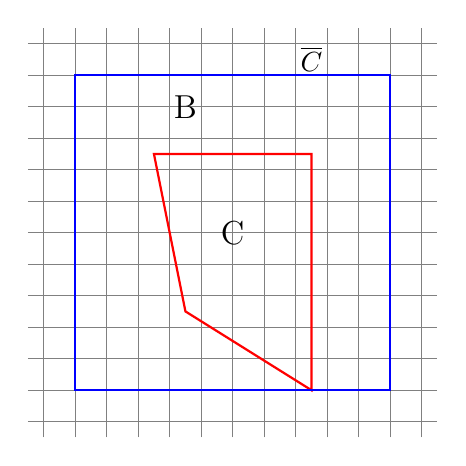
\begin{tikzpicture}[scale=0.20]
		% draw the grid
		\draw[step=2cm,gray,very thin] (-13,-13) grid (13,13);
		% draw the polygonal curve
		\draw[red,thick] (-3,-5) -- (-5,5) -- (5,5) -- (5,-10) -- cycle;
		\draw[blue,thick] (-10,-10) -- (-10,10) -- (10,10) -- (10,-10) -- cycle;
		\node at (0,0) {\large {C}};
		\node at (5,11) {$\large{\overline C}$};
		\node at (-3,8) {\blue{\large{B}}};
	\end{tikzpicture}
	\caption{Los cortes los ilustramos tachando las aristas que pertenecen a $\delta C$.}
	\end{figure}


Una propiedad fundamental de los cortes en estos grafos es que fijada una arista solo hay finitos cortes que tienen a esta arista dentro de su borde.	
\begin{lema}\label{lema_finitos_kcortes}
	Sea $\Gamma$ un grafo conexo y localmente finito.
	Sea $S \subset V$ un conjunto finito y $k\ge 1$.
	Entonces existen finitos $k$-cortes $C$ con $\beta C \cap S \neq \emptyset$.
\end{lema}	

\begin{proof}
	Primero notemos que nos alcanza con ver los cortes $C$ que tienen una arista fija $(x,y) \in \delta C$.
	Si vemos que estos son finitos entonces como tenemos finitos $x \in S$ y cada vértice tiene finitas aristas dado que el grafo es localmente finito entonces tenemos que la cantidad de $k$ cortes sería finita.
	Consideremos entonces que $S = \{ x \}$ porque los otros casos se siguen de este.
	
	Vamos a probarlo por inducción en $k$.
	
	En el caso base tenemos que $\delta C = (x,y)$.
	En este caso tenemos que solo puede haber finitos cortes (al menos tantos como aristas salen del vértice $x$).
	
	Ahora veamos el paso inductivo.
	Como suponemos que es un $k$-corte con $k \ge 2$ al menos tenemos una arista sea esta $(x,y)$.
	Notemos que si $\Gamma \setminus (x,y)$ no está conectado entonces no puede haber un corte $C'$ tal que $(x,y) \in \delta C'$ y que cumpla que $|\delta C'| \ge 2$.
	Esto nos dice que nos queda ver el caso que $\Gamma \setminus (x,y)$ sigue siendo conexo. 
	Al seguir siendo conexo debe existir un camino de vértices $\gamma$  en $ \Gamma \setminus (x,y) $ tal que $\gamma = x_0 x_1 \dots x_{n}$ con $x_0 = x$ y con $x_{n} = y$.
	Todos estos $k$-cortes $C$ que estamos considerando tienen que cumplir que alguno de las aristas $(x_i,x_{i+1}) \in  \gamma \cap \delta C$.
	Caso contrario tendríamos que para todo $x_i \in \gamma$ vale que $x_{i} \in C$ o bien $x_i \in \ol C$ contradiciendo que $(x,y) \in \delta C$.
	Finalmente como todo $k$-corte que contiene a $(x,y)$ restringido a $\gamma$ resulta ser un $(k-1)$-corte tenemos que al ser estos finitos por la hipótesis inductiva que la cantidad de $k$-cortes es finita tal como queríamos ver.
	
\end{proof}
	
\begin{deff}
	Dado $\Gamma$ un grafo conexo diremos que un camino simple $\alpha$ es un \emph{rayo} si
	\[
		\alpha = v_0 \dots v_{n} \dots
	\]	
	Diremos que es un \emph{camino infinito} si
	\[
		\alpha =  \dots v_{-n} \dots v_0 \dots v_{n} \dots 
	\]
\end{deff}	
	

Una primera observación es que dado un corte $C$ tal que $C$ es infinito y $\ol C$ también lo es, podemos armarnos un camino infinito $\alpha$ tal que $|\alpha \cap C| = \infty = |\alpha \cap \ol C|$.
Fijemos dos vértices $u \in C$ y $v \in \ol C$ de manera que $(u,v) \in \delta C$.
Por el lema de König  tenemos un rayo infinito dentro de $C$.
Si este rayo no pasa por el vértice $u$ nos tomamos un camino simple finito que una $u$ con el origen de este rayo llamemos a este vértice $u_{0}$.
Consideremos entonces el primer vértice del rayo que interseca a este camino, sea este $u_{1}$.
Si consideramos la concatenación de este camino finito hasta $u_{1}$ y luego la continuación del rayo a partir de $u_{1}$ obtenemos el rayo $\alpha \cap C$.
Para obtener la otra parte y así llegar a tener un camino infinito $\alpha$ hacemos lo mismo a partir del vértice $v \in \ol C$ y luego concatenamos estos caminos con el vértice $(u,v)$ para así llegar a un camino infinito $\alpha$. 

No necesariamente vale la vuelta.
Esto es que si tenemos un camino infinito $\alpha$ y un corte $C$ entonces el corte cumple que $|\alpha \cap C| = \infty = |\alpha \cap \ol C|$.

Esto nos lleva a dar la siguiente definición.

\begin{deff}
	Sea $\alpha$ un camino infinito.
	Definimos el conjuntos de cortes del camino como 
	\[
		{\cal C}(\alpha) = \{ C \subset V(\Gamma) \mid  C \ \text{es un corte y} \ |\alpha \cap C| = \infty = |\alpha \cap \ol C| \}
	\] 
\end{deff}

Una manera equivalente de escribir esta definición es que ${\cal C}(\alpha) \neq \emptyset$ si y solo sí existe un corte $C$ de manera que $\alpha \setminus \delta C$ tiene dos componentes conexas infinitas.


\begin{deff}
	Dado $\alpha$ camino infinito definimos el conjunto de sus cortes mínimos como
	\[
		\cam = \{  C \in \ca : |\delta C| \ \text{es mínimo}  \}
	\]
	
	Dado un grafo $\Gamma$ definimos el conjunto de sus cortes mínimos como 
	\[
		{\cal C}_{\text{min}} = \bigcup \{ \cam : \alpha \ \text{es un camino infinito}  \}
	\]
\end{deff}

\begin{deff}
	Dos cortes $C,D \in V(\Gamma)$ están anidados si vale alguna de las cuatro inclusiones $C \subseteq D, C \subseteq \ol D, \ol C \subseteq \ol D, \ol C \subseteq D$.
	Los conjuntos $C \cap D, C \cap \ol D, \ol C \cap D, \ol C \cap \ol D$ los llamamos las esquinas.
\end{deff}

\begin{lema}
	Dos cortes $C,D$ están anidados si y solo si alguna de las cuatro esquinas es vacía.
\end{lema}
\begin{proof}
	Para la ida supongamos que $C \subseteq D$ luego tiene que valer que $\ol C \cap \ol D = \emptyset$.
	Para la vuelta si por ejemplo $C \cap D = \emptyset$ como vale que $C = C \cap D \cup C \cap \ol D$ esto nos dice que $C \subseteq \ol D$.
\end{proof}

\begin{lema}
	Dado $C$ corte y $k \in \NN$ tenemos que 
	\[
		| \{  D : C, D \ \text{no están anidados y} \ D \ \text{es un k-corte}   \} | < \infty
	\]
\end{lema}
\begin{proof}
	Por el lema anterior \ref{lema_finitos_kcortes} tenemos finitos $k$-cortes tales que intersecan a $\beta C$ dado que este es un conjunto finito.
	
	Esto nos dice que debemos mirar los casos que $\beta C \subseteq D$.
	Si $C,D$ no estuvieran anidados tendríamos que $C \cap \ol D \neq \emptyset \neq \ol C \cap \ol D$.
	Esto nos diría que podríamos tomarnos un camino entre $c_0 \in C \cap \ol D$ y $c_1 \in \ol C \cap \ol D$ tal que esté contenido en $\ol D$.
	Esto es una contradicción porque este camino tendría que pasar por $\beta C$ y sabemos que $\beta C \subseteq D$.

	En conclusión tenemos que todos los $k-$cortes no anidados tienen que intersecar a $\beta C$ y estos son finitos.			
\end{proof}

Esto nos dice que la siguiente definición es correcta.

\begin{deff}
	Dado $\Gamma$ grafo conexo y localmente finito, $C$ un corte y $k \in \NN$ constante definimos el siguiente número natural,
	\[
		m_k(C) = | \{  D : C, D \ \text{no están anidados y} \ D \ \text{es un k-corte}   \} |. 
	\]
\end{deff}

Consideremos ahora que el grafo $\Gamma$ es accesible y su constante es $k$.
En este caso notaremos para cada corte $C$ el siguiente valor
\[
	m(C) = m_k(C).
\]

\section{Cortes óptimos.}

Así como definimos cortes mínimos ahora vamos a definir cortes óptimos que serán un subconjunto de ellos.

\begin{deff}
	Dado $\alpha$ camino infinito sea
	\[
		m_\alpha = \min \{ m(C) : C \in \cam \}.
	\]
	De esta manera los cortes óptimos del camino $\alpha$ serán
	\[
		\copta = \{ C \in \cam : m(C) = m_\alpha  \}
	\]
	y el conjunto de los cortes óptimos análogamente será el conjunto que contenga a todos ellos
	\[
		\copt = \bigcup \ \{ \copta : \alpha \ \text{es un camini bi-infinito}  \}.
	\]
\end{deff}

El siguiente es el resultado central y más importante de los cortes óptimos.

\begin{teo}\label{teo_copt_anidados}
	Todo par de cortes óptimos $C,D \in \copt$ está anidado.
\end{teo}
\begin{proof}
	Tenemos dos caminos $\alpha$, $\beta$ tales que $C \in \copt(\alpha)$ y $D \in \copt(\beta)$.
	Supongamos que $m_{\alpha} \ge m_{\beta}$.
	Esta suposición nos dice que en el caso que $D \in {\cal C}_{\text{min}}(\alpha)$ luego por ser óptimo para $\beta$ resulta que $D \in \copt(\alpha)$.
	Esto fuerza a que $m_{\alpha} = m_{\beta}$, por lo tanto tenemos que en este caso en particular podemos considerar simplemente el camino $\alpha$ y olvidarnos de $\beta$.
	
	La idea de la demostración es suponer que estos dos cortes no están anidados y llegar a una contradicción.
	Para esto queremos encontrar cortes $E, E' \in \copt$ de manera que hagan valer la siguiente desigualdad:
	\[
		m(E) + m(E') < m(C) + m(D).
	\]   
	La validez de esta desigualdad nos diría que alguno de los dos cortes $C,D$ no es óptimo tal como supusimos.
	
	Consideremos el caso que $\alpha = \beta$.
	Afirmamos que hay dos esquinas de $C,D$ tales que contienen infinitos vértices de $\alpha$.
	Caso contrario si solamente alguna de las esquinas, supongamos $C \cap D$ tiene infinitos vértices entonces tendríamos que $|\alpha \cap \ol C| < \infty$ negando que $C \in {\cal C}(\alpha)$.
	Cambiando los nombres a los cortes, sean estas esquinas $E = C \cap D$ y $E' = \ol C \cap \ol D$.
	
	Consideremos ahora el caso que $\alpha$ y $\beta$ son caminos distintos.
	Afirmamos que hay una esquina $K$ tal que $|K \cap \alpha| < \infty$ y tal que $|K \cap \beta| < \infty$.
	Caso contrario tendríamos que $D \cap \alpha = D \cap C \cap \alpha  \cup D \cap \ol C \cap \alpha$ e idénticamente para $\ol D$, obteniendo así que $D \in \copt(\alpha)$.
	Por la primera observación esto nos diría que $\alpha = \beta$ así que este caso queda descartado.
	Consideremos las esquinas $E,E'$ que son adyacentes a $K$.
	Notemos que estas esquinas cumplen que $|E \cap \alpha| = \infty$ y que $|E' \cap \beta| = \infty$ caso contrario negaríamos que estos cortes separan en dos a los caminos.
	Sin pérdida de generalidad supongamos que $E = C \cap D$ y que $E' = \ol C \cap \ol D$.
	
	Nuestros posibles candidatos a cortes óptimos son $E,E'$ pero en principio no sabemos si son cortes siquiera.
	Sea $F$ componente conexa de $E$ tal que $|F \cap \alpha| = \infty$.
	Notemos que $\ol C \cup \ol D \subseteq \ol F$ por lo tanto tenemos que $|\ol F \cap \alpha|=\infty$.
	Más aún podemos ver que $\ol F$ es conexo.
	Para eso consideremos $v,w \in \ol F$.
	Si ambos vértices están en un mismo corte ya está porque es conexo por lo tanto tenemos un camino que los une y no toca a $F$.
	Si no están en un mismo corte, como podría ser que $v \in C \cap \ol D$ y $w \in \ol C \cap D$ luego usando la conexión de $\ol D$ y de $\ol C$ podemos unir ambos con algún vértice en $\ol C \cap \ol D$ y así vemos que es conexo.
	Con esto concluimos que $F$ es un corte que separa en dos partes a $\alpha$.
	Hacemos algo similar para construirnos un corte $F' \subseteq E'$ que separe en dos partes a $\beta$.
	
	Veamos ahora que $E=F$ y que $E' = F'$.
	Para eso consideremos los bordes. 
	Por como elegimos a $E$ tenemos que $\delta E \subseteq \delta D \cup \delta C$ y similarmente para $E'$ concluyendo así que $\delta E \cup \delta E' \subseteq \delta D \cup \delta C$.
	De esto se sigue la siguiente desigualdad,
	\begin{align*}
		|\delta E \cup \delta E'| & \le |\delta C \cup \delta D| \\
		|\delta E| + |\delta E'| - |\delta (E \cap E')| & \le |\delta C| + |\delta D| - |\delta (C \cap D)|
	\end{align*}
	y usando que las intersecciones están acotadas obtenemos finalmente la ecuación,
	\[
		|\delta E| + |\delta E'| \le |\delta C| + |\delta D|.
	\]
	Por otro lado como $F$ es una componente conexa de $E$ tenemos que $\delta F \subseteq \delta E$ y similarmente para el caso de $F'$ dentro de $E'$.
	Esto nos dice que en definitiva tenemos estas desigualdades,
	\[
		|\delta F| \le  |\delta E|, \ |\delta F'| \le |\delta E'| 
	\]
	y como $F$ es un corte en ${\cal C}(\alpha)$ y $F'$ es un corte en ${\cal C}(\beta)$ obtenemos finalmente que $|\delta F| = |\delta E|$ y que $|\delta F'| = |\delta E'|$ concluyendo así que $E=F$ y que $E'=F'$.
	Así vimos que tanto $E$ como $E'$ son cortes mínimos.
	Queremos ver ahora que son óptimos.
	
	Para esto probaremos primero que si $F$ es un corte anidado con $C$ o con $D$ entonces está anidado con $E$ o con $E'$.
	Separamos en dos casos que son simétricos.
	Si $F \cap C = \emptyset$ entonces $F \cap E= \emptyset$ y similarmente si $F \cap \ol C = \emptyset$ entonces $F \cap E' = \emptyset$.
	Esto nos va a decir que todos los cortes que estén anidados con alguno de los dos cortes originales va a estar anidado con alguno de los dos propuestos.
	No tenemos garantizada la desigualdad de $m(E) + m(E') < m(C) + m(D)$ porque nos faltaría el caso que algún corte no esté anidado con $C$ y con $D$ a la vez.
	Entonces supongamos que $F$ no está anidado con $C$ ni con $D$ y queremos ver que no lo está con $E$ ni con $E'$.
	Tenemos cuatro casos a analizar.
	\begin{enumerate}
		\item $C \subseteq F$ y $D \subseteq \ol F$.
		Este caso está descartado porque tendríamos que $E=\emptyset$ y sabemos que $E$ es infinito. 
		\item $\ol C \subseteq F$ y $\ol D \subseteq \ol F$.
		Similar al caso anterior tendríamos que $E' = \emptyset$ y es una contradicción.
		\item $\ol C \subseteq F$ y $D \subseteq \ol F$.
		Esto nos dice que $E \subseteq \ol F$ y que $E' \subseteq F$.
		\item $ C \subseteq F$ y $D \subseteq \ol F$.
		Esto nos dice que $E \subseteq F$ y que $E' \subseteq \ol F$.
	\end{enumerate}
	En definitiva llegamos a la siguiente desigualdad,
	\[
		m(E) + m(E') \le m(C) + m(D)
	\]
	pero nosotros queremos ver que es estricta para terminar de probar este teorema.
	Para eso notemos que $C$ está anidado con $E$ puesto que $\ol C \cap E = \ol C \cap C \cap D = \emptyset$.
	Idénticamente vemos que está anidado con $E'$.
	Pero por suposición tenemos que $C$ y $D$ no están anidados así que tenemos una desigualdad estricta y por lo tanto llegamos a una contradicción de suponer que los cortes $C,D$ no están anidados.
\end{proof}

\section{Árbol de estructura.}

\begin{deff}
	Un grafo $\Gamma$ es \emph{accesible} si existe $k \in \NN$ de manera que todo camino infinito $\alpha$ cumple que ${\cal C}(\alpha) = \emptyset$ o bien ${\cal C}(\alpha)$ contiene un $k$-corte.
\end{deff}



Todos los grafos que vamos a considerar a partir de ahora son accesibles.
Veamos que los caminos óptimos resultan ser un poset discreto con la inclusión en este caso.
En esta subsección vamos a construir un árbol a partir de ciertos cortes de un grafo de manera que este árbol nos de una descomposición.

\begin{lema}\label{lema_intermedios}
	Si $C,D \in \copt$ luego 
	\[
	|\{ E \in \copt : C \subseteq E \subseteq D \}| < \infty
	\]
\end{lema}
\begin{proof}
	Tomemos un camino $\gamma$ tal que salga de $c \in C$ y termine en $d \in \ol D$.
	
	Si $E$ es un corte luego tiene que separar a $\gamma$ caso contrario tendríamos que $d \in E \cap \ol D$.
	Como el grafo que estamos considerando es accesible sabemos que $E \in \copt$ implica que $E$ es un $k$-corte.
	Si ahora usamos el lema \ref{lema_finitos_kcortes} con el conjunto finito $\gamma$ esto nos dice que solo existen finitos cortes $E$ que cumplen lo pedido.
\end{proof}

Ahora vamos a definir la siguiente relación sobre los cortes óptimos.

\begin{deff}
	Dos cortes $C \sim D \in \copt$ si y solo sí
	\[
		C = D \ \text{o bien} \ \ol C \subsetneq D \ \text{y} \ \forall E \in \copt : \ol C \subsetneq E \subseteq D \implies D = E
	\]
\end{deff}

\begin{prop}
	La relación $\sim$ es de equivalencia.
\end{prop}
\begin{proof}
	Por como la definimos es clara que es reflexiva.
	Para ver que es simétrica notemos que si $C \sim D$ y son cortes distintos entonces  
	\[
		\ol C \subsetneq D \implies \ol D \subsetneq C
	\]
	por lo tanto volviendo a tomar complemento obtenemos que
	\[
	\forall E \in \copt : \ol C \subsetneq E \subseteq D \implies D = E \implies \forall E \in \copt : \ol D \subsetneq E \subseteq C \implies C = E.
	\]
	
	Finalmente nos queda ver que la relación resulta ser transitiva.
	Esto es que para ciertos cortes óptimos tenemos que $C \sim D$, $D \sim E$ y queremos ver que $C \sim E$.
	Una primera observación que podemos hacer es que $\emptyset \neq \ol D = C \cap E$.
	Esto sale de que  
	
	Por el teorema \ref{teo_copt_anidados} tenemos que $C,E$ están anidados.
	Veamos que sucede en los cuatro posibles casos.
	\begin{itemize}
		\item $C \subseteq E$. 
		Tenemos que $\ol D \subsetneq E$ con $\ol D \subsetneq F \subseteq E$ y esto implica que $F=E$.
		Si tomamos $F = C$ entonces obtenemos lo que queríamos ver.
		\item $E \subseteq C$ análogo al caso anterior.
		\item $E \subseteq \ol C$ contradice que $C \cap E \neq \emptyset$.
		\item $\ol C \subseteq E$.
		Como $C \cap E \neq \emptyset$ esto nos dice que $\ol C \subsetneq E$ por lo tanto tenemos que si $F \in \copt$ luego	$\ol C \subsetneq F \subseteq E$ queremos ver que $F=E$.
		Lo separamos en cuatro casos nuevamente gracias al teorema \ref{teo_copt_anidados} dado que $F$ debe estar anidado con $D$.
		\begin{itemize}
			\item $D \subseteq F$.
			Esto nos dice que $D \subseteq E$ pero por lo visto tenemos que $\ol D \subseteq E$ y esto es una contradicción porque al ser $E$ un corte no puede ser todo el conjunto de vértices $V(\Gamma)$.
			\item $D \subseteq \ol F$. 
			Esto nos dice que $F \subseteq \ol D$ y por lo tanto tenemos $\ol C \subsetneq F \subseteq \ol D$ pero esto nos dice que $\ol C \subseteq \ol D$ y como $\ol D \subseteq C$ llegamos a una contradicción.
			\item $\ol D \subseteq F$.
			Usamos que $D \sim E$ por lo tanto concluimos que $F=E$ tal como queríamos ver.			
			\item $\ol D \subseteq \ol F$.
			Esto nos dice que $\ol C \subsetneq F \subseteq D \subseteq E$ por lo tanto obtenemos que $F = D$ o bien contradecimos que $C \sim D$.
		\end{itemize}
	\end{itemize}
\end{proof}

\begin{deff}
	Sea $\Gamma$ un grafo conexo, accesible y localmente finito y sea $\copt$ el conjunto de sus cortes óptimos.
	El árbol de estructura $T(\copt)$ de un grafo $\Gamma$ es el siguiente grafo.
	\begin{align*}
		V(T(\copt)) &= \{ [C] : C \in \copt \} \\
		E(T(\copt)) &= \{ ([C], [\ol C]) : C \in \copt   \}
	\end{align*}
\end{deff}

\begin{obs}
	Por nuestra construcción el árbol de estructura no es localmente finito.
	El grado de cada vértice $[C] \in V(T(\copt))$ está acotado por el órden de la clase de equivalencia de $C$ y éste podría ser infinito.
\end{obs}

\begin{prop}
	El grafo $T(\copt)$ es un árbol.
\end{prop}

\begin{proof}
	Debemos ver que es acíclico y conexo.
	
	Primero veamos que no tiene ciclos.
	Supongamos que $\gamma$	es un ciclo y aparte tomesmolo para que sea simple luego tendría la siguiente forma
	\[
		[C_0], [C_1], [C_2], \dots [C_{n}], [C_0]
	\]
	donde $\ol C_{i} \sim C_{i+1}$ para todo $i=1 \dots n$.
	Por otro lado al ser simple nos dice que $C_{i-1} \nsim C_{i+1}$ caso contrario tendríamos que el camino tiene backtracking.
	Esto nos da una cadena de inclusiones
	\begin{equation}\label{eq:inclusiones}
			C_0 \subsetneq C_1 \subsetneq \dots C_{n-1}
	\end{equation}
	tal que $\ol C_{n-1} \sim C_n \sim \ol C_0$.
	Veamos que no puede haber una arista $(C_{n-1}, C_0)$.
	Si la hubiera tendría que valer alguna de estas dos inclusiones:
	\begin{enumerate}
		\item $\ol C_{n-1} \subsetneq C_0$.
		Usando \ref{eq:inclusiones}, esto nos diría que $\ol C_{n-1} \subseteq C_{n-1}$ que es una contradicción.
		\item $\ol C_{0} \subsetneq C_{n-1}$.
		Nuevamente usando las inclusiones \ref{eq:inclusiones} llegaríamos a que $V(\Gamma) = C_0 \cup \ol C_0 \subseteq C_{n-1} \subsetneq V(\Gamma)$ que también es una contradicción.
	\end{enumerate}
	Por lo tanto el grafo resulta ser acíclico.
	
	Veamos ahora que es conexo.
	Sean $[C], [D] \in V(T(\copt))$, veamos de construir un camino entre ellos.
	Por el teorema \ref{teo_copt_anidados} tenemos que necesariamente están anidados.
	Sin pérdida de generalidad podemos suponer que $C \subseteq D$ dado que
	\[
	([C], [\ol C]), ([D],[\ol D]) \in E(T(\copt))
	\]
	Por el lema \ref{lema_intermedios} sabemos que hay finitos cortes $E$ intermedios.
	Tomemos entonces una sucesión creciente no refinable de cortes de manear que llegamos 
	\[
		C=C_0 \subsetneq C_1 \subsetneq \dots C_n = D
	\]
	luego por como tomamos estos cortes obtenemos que $\ol C_i \sim C_{i+1}$ por lo tanto obtenemos el siguiente camino $[C],[C_1], \dots, [C_{n-1}],[D]$ en el grafo $T(\copt)$ probando así que es conexo.	
\end{proof}

\section{Acciones sobre el árbol de estructura.}

Sea $\Gamma$ un grafo accesible, conexo y localmente finito tal que $\aut(\Gamma)$ actúa con finitas órbitas sobre este grafo.

Una primera observación que podemos hacer es que $\aut(\Gamma)$ actúa sobre $\copt$.
Para eso notemos que si $C$ es un corte luego si $\varphi \in \aut(\Gamma)$ tenemos que $\varphi(C)$ es conexo y no vacío. 
Por otro lado al ser un morfismo del grafo $\Gamma$ obtenemos que $\ol{\varphi(C)} = \varphi(\ol C)$ por lo tanto su complemento sigue siendo conexo.
Al ser un automorfismo tenemos que $\varphi(\beta C) = \beta (\varphi C)$ y por este motivo tenemos que $|\varphi (\beta C)| = |\beta (\varphi C)|$ y esto nos dice que manda $k$-cortes en $k$-cortes.
Veamos que manda un corte minimal en uno minimal. 
Para eso si $C \in {{\cal C}}_{\text{min}}(\alpha)$ para cierto camino infinito $\alpha$ luego notemos que $\varphi(\alpha)$ es otro camino infinito y por ser un automorfismo obtenemos que $\varphi(C) \in {\cal C}_{\varphi(\alpha)}$.
Similarmente tenemos que si $C$, $D$ no están anidados luego necesariamente $\varphi(C)$ y $\varphi(D)$ no están anidados tampoco.
Caso contrario si $\varphi(C) \cap \varphi(D) = \emptyset$ luego tendríamos que al ser $\varphi \in \aut(\Gamma)$ que preserva las intersecciones y tiene una inversa por lo que $C \cap D = \emptyset$ y esta es la contradicción.
Juntando todo nos dice que $\aut(\Gamma)$ actúa sobre los cortes óptimos.

Esta acción no solo es sobre el conjunto $\copt$ sino que podemos ver que actúa por medio de morfismos de grafos sobre el árbol de estructura $T(\copt)$.
Para esto notemos que si $C \sim D \in \copt$ son cortes óptimos relacionados luego tenemos que para todo $\varphi \in \aut(\Gamma)$ vale que $\varphi(C) \sim \varphi(D)$.
Para eso notemos que si $\ol C \subsetneq E \subset D$ implica que $E = D$ luego si tenemos que
\[
	\ol {\varphi(C)} \subsetneq E \subset \varphi(D) \iff C \subsetneq \varphi(E) \subset D
\]  
donde usamos que $\varphi$ es un automorfismo y que actúa sobre los cortes óptimos.
Esto nos dice que la acción dada por $\varphi([C]) = [\varphi (C)]$ está bien definida y por lo tanto actúa sobre los vértices.
Para ver que actúa sobre las aristas notemos que al ser un morfismo de grafos y por actúar sobre los vértices que $[\ol \varphi(C)] = [\varphi (\ol C)]$.

\begin{lema}\label{lema_finitas_orbitas}
	Sea $\Gamma$ un grafo accesible.
	Si $\aut(\Gamma)$ actúa con finitas órbitas sobre $\Gamma$ luego actúa con finitas órbitas sobre $\copt$ y sobre el árbol de estructura $T(\copt)$.
\end{lema} 
\begin{proof}
	Veamos primero que actúa con finitas órbitas sobre $\copt$.
	Para eso tenemos que existe $A \in V(\Gamma)$ dominio fundamental finito de la acción de $\aut(\Gamma)$ sobre $\Gamma$.
	Por lo tanto todo corte se puede tomar alguno que esté en su misma órbita, llamesmolo $C$ de manera que $C \cap A \neq \emptyset$.
	Como el grafo es accesible todo corte óptimo es un $k$-corte para un cierto $k$.
	Por el resultado \ref{lema_finitos_kcortes} tenemos que hay finitos cortes posibles por lo tanto tenemos que hay finitas órbitas posibles para esta acción.
	
	Para ver que son finitas las órbitas sobre el árbol de estructura notemos que al ser $V(T(\copt))$ isomorfo a un cociente de $\copt$ luego tenemos que en particular las órbitas sobre el árbol de estructura también tienen que ser finitas.
\end{proof}

\begin{obs}
	Un caso particular que nos interesa es cuando el grafo $\Gamma$ es el grafo de Cayley para cierto \fg $G$.
	En este caso tenemos que $G$ es un subgrupo de $\aut(\Gamma)$ y como $G$ tiene una única órbita se sigue que $|\aut(\Gamma)/\Gamma| = 1$ de manera que en particular actúa con finitas órbitas.		
\end{obs}

Nuestro objetivo ahora es entender cómo es la acción sobre el árbol de estructura. 
Lo primero que vamos a buscar entender es cómo son los estabilizadores de esta acción.

\begin{lema}\label{lema_nlC_cap_olC_conexo}
	Existe $l \in \NN$ de manera que $N^l(C) \cap \ol C$ es conexo para todo $C \in \copt$.
\end{lema}
\begin{proof}
	Primero consideremos algún $C \in \copt$ y después veamos de extender este resultado para todos los cortes óptimos.
	
	Para empezar sea $v \in \delta C \cap \ol C$ y consideremos $l' = \max  \{d(v,w) \ | \ w \in \delta C\}$.
	Como $\ol C$ es conexo tenemos que $N^{l'+1}(C) \cap \ol C$ resulta ser conexo.
	Esto porque si $w,w' \in N^{l'+1}(C) \cap \ol C$ luego su distancia a $C$ está acotada por $l'+1$ por lo tanto existe un camino que lo une con $C$ menor a esa longitud.
	Si ambos pasan por $u,u' \in \delta C \cap \ol C$ vértices que estén en el borde luego por nuestra elección de $l'$ tenemos que $d(u,v) \le l'$ y que $d(u',v) \le l'$ concluyendo así que $N^{l'+1}(C) \cap \ol C$ es conexo.
	
	Para finalizar la demostración observemos que por el lema anterior \ref{lema_finitas_orbitas} tenemos finitas órbitas de cortes óptimos.
	Para cada representante de órbita $C_i \in \copt$ donde $i=1,\dots,n$ podemos tomar $l_i \in \NN$ de manera que nos sirva y finalmente tomando $l = \max_{i=1,\dots,n} l_i$ vemos que nos sirve para todos los representantes de órbitas y así para todos los cortes óptimos.
\end{proof}
\begin{obs}
	En particular tenemos que $|N^l(C) \cap \ol C|<\infty$ dado que si $v \in N^l(C) \cap \ol C$ luego existe $w \in \beta C \cap C$ tal que esté en el camino que une $v$ con $C$.
	Esto nos dice que resulta ser el conjunto $N^l(\beta C  \cap C) \cap \ol C$ que sabemos que es finito porque $\beta C \cap C$ es finito por ser un corte.
\end{obs}
Ahora definimos un objeto que nos va a ayudar a entender como son estos estabilizadores.

\begin{deff}
	Sea $\Gamma$ un grafo tal que $\aut(\Gamma)$ actúa con finitas órbitas sobre $\copt$.
	Sea $l \in \NN$ tal que $N^l(C) \cap \ol C$ es conexo para todo $C \in \copt$.
	El bloque asignado a $[C] \in V(T(\copt))$ está definido como
	\[
		B([C]) = \bigcap_{D \sim C} N^l (D)
	\]	
\end{deff}

Veamos que estos bloques no son vacíos.

\begin{lema}
	Tenemos la siguiente igualdad de conjuntos,
	\[
		B([C]) = \bigcap_{D \sim C} D \cup \bigcup_{D \sim C} N^l(D) \cap \ol D
	\]
\end{lema}

\begin{proof}
	Veamos las dos inclusiones.
	
	\begin{itemize}
		\item \textbf{$(\subseteq)$}. 
		Sea $v \in B([C])$. 
		Si $v \in \bigcap_{D \sim C} D$ ya está. 
		Caso contrario tenemos que debe existir $D \in [C]$ tal que $v \in N^l(D) \cap \ol D$ y por lo tanto queda probada esta inclusión.
		\item \textbf{$(\supseteq)$} 
		Nos alcanza con ver que $ N^l(D) \cap \ol D \subseteq B([C])$ para todo $D \in [C]$.
		Para eso notemos que al estar en la misma clase de equivalencia tenemos que 
		\[
			N^l(D) \cap \ol D \subseteq \ol D \subsetneq C \subseteq N^l(C)
		\]
		terminando de probar esta inclusión y así obteniendo la igualdad de conjuntos.
	\end{itemize}
\end{proof}

Estos bloques aparte cumplen que son conexos.

\begin{lema}\label{lema_conexion_B(C)}
	Existe una constante $\lambda \in \NN$ tal que para todo $C \in \copt$ y todo $S \subseteq B([C])$ tenemos que: 
	Cuando dos vértices $u,v \in B([C]) \setminus N^l(S)$ se pueden conectar por algún camino en $\Gamma \setminus N^l(S)$ entonces se pueden conectar por algún camino en $B([C]) \setminus S$. 
\end{lema}

\begin{proof}
	% Agregar dibujito.
	Consideremos $\lambda = \max \{ d(u,v) \ | \ D \in \copt, u,v \in N^l(D) \cap \ol D  \}$ que sabemos existe porque tenemos finitas órbitas de cortes óptimos tal como en el lema \ref{lema_nlC_cap_olC_conexo}. 	
	
	Vamos a probarlo por inducción en la longitud del camino.
	Sea $\gamma$ camino en $\Gamma \setminus N^{\lambda}(S)$ tal que une $u$ con $v$.
	Queremos ver de acortar este camino usando que $N^{\lambda}(D) \cap \ol D \subseteq B([C])$ es conexo.
	Si $\gamma \subseteq B([C])$ ya está entonces consideremos el primer vértice $v_m$ de $\gamma$ tal que $v_m \notin B([C])$ y esto quiere decir que para cierto $D \in [C]$ tenemos que $v_m \notin N^l(D)$.
	Esto nos dice que $v_{m-1} \in N^l(D) \cap \ol D$ caso contrario tendríamos que $v_m \in N^l(D)$.
	
	Consideremos ahora el primer vértice $v_n$ de $\gamma$ con $n > m$ tal que $v_n \in N^l(D)$.
	Por ser el primer vértice tenemos que en particular que $v_n \in N^l(D) \cap \ol D$.
	Dado que $N^l(D) \cap \ol D$ es conexo tenemos un camino que une $v_{m-1}$ con $v_m$ tal que está contenido en $N^l(D) \cap \ol D$ y en particular está contenido en $B([C])$.
	Este camino evita $S$ porque como $d(v_n,v_m) \le \lambda$ esto nos diría que $d(v_n,S) \le \lambda$ contradiciendo que el camino $\gamma$ está contenido en $\Gamma \setminus N^{\lambda}(S)$.	
\end{proof}


\begin{obs}
	Como corolario del resultado anterior obtenemos que para todo $C \in \copt$ vale que $B([C])$ es conexo.
	Esto porque podemos tomar $S = \emptyset$.
\end{obs}

\begin{lema}\label{lema_accion_vecinos}
	Sea $D$ corte y sea $g \in G$ entonces vale la siguiente igualdad de conjuntos,
	\[
		g \cdot N^l(D) = N^l(g \cdot D).
	\]
\end{lema}

\begin{proof}
	Veamos las dos contenciones.
	
	\begin{itemize}
		\item $(\subseteq)$. 
		Sea $v \in N^l(D)$ luego existe $w \in D$ tal que $d(v,w) \le l$.
		Como multiplicar por $g$ es un automorfismo manda vértices adyacentes en vértices en adyacentes, en particular no aumenta la distancia.
		Esto es que $d(g\cdot v,g\cdot w) \le l$ concluyendo así que $g \cdot v \in N^l(g \cdot D)$  
		\item $(\supseteq)$.
		Si $v \in N^l(g\cdot D)$ luego tenemos que debe existir $w \in D$ tal que $d(g \cdot w, v) \le l$.
		Ahora como multiplicar por $g$ es un automorfismo con inversa multiplicar por $g^{-1}$ obtenemos que 
		\[
			d(g^{-1} \cdot v, w) \le l \implies v \in g\cdot N^l(D).
		\]
	\end{itemize}
\end{proof}

\begin{lema}\label{lema_g_actua_b(C)}
	Sea $g \in G_{[C]}$ luego tenemos que $g \cdot B([C]) = B([C])$.
\end{lema}
\begin{proof}
	Si $v \in B([C])$ luego $v \in \bigcap_{C \sim D} N^l(D)$.
	Por lo tanto usando que multiplicar por $g$ es un automorfismo del grafo obtenemos la siguiente igualdad
	\[
		g\cdot v \in \bigcap_{C \sim D} g \cdot N^l(D)
	\]
	por lo que por el lema \ref{lema_accion_vecinos} concluímos que 
	\[
		g\cdot v \in \bigcap_{C \sim D}   N^l(g\cdot D).
	\]	
	
	Por nuestra hipótesis tenemos que $g \cdot C \sim C$ luego si $D \sim C$ obtenemos que dado que la acción de $G$ está bien definida sobre $T(\copt)$ que $g\cdot D \sim g\cdot C \sim C$ tal como queríamos ver.		
	
\end{proof}

\begin{lema}\label{lema_accion_b(C)}
	Sea $\Gamma$ un grafo conexo, localmente finito y accesible tal que $G$ actúa sobre $\Gamma$ con finitas órbitas.
	Entonces $G_{[C]}$ actúa con finitas órbitas sobre $B([C])$.
\end{lema}
\begin{proof}
	Podemos ver que $G_{[C]}$ actúa con finitas órbitas sobre $[C]$.
	La acción es la restricción de la acción de $G$ que sabemos que tiene finitas órbitas y está bien definida porque si $C \sim D$ luego si $g \cdot C \sim C$ esto nos dice que $g \cdot D \sim g \cdot C \sim C$.
	
	Ya sabemos que $G_{[C]}$ actúa sobre $B([C])$ justamente por el lema previo \ref{lema_g_actua_b(C)}.
	Queremos ver que lo hace con finitas órbitas.
	
	Para eso vamos a ver que existe $m \in \NN$ tal que para todo $v \in B([C])$ existe un corte $D$ que cumple las siguientes dos propiedades:
	\begin{enumerate}
		\item $D \sim C$.
		\item $d(v,\beta D) \le m$.
	\end{enumerate}
	
	Como $G$ actúa con finitas órbitas sobre $\copt$ en particular lo hace sobre el subconjunto $\bigcup_{D \sim C} \beta D$.
	Dado que el grafo resulta ser localmente finito tenemos que entonces todo $v \in B([C])$ tendría que estar en la órbita de alguno de estos finitos elementos.
	
	Probemos entonces que existe tal corte $D$.
	Sea $v \in B([C])$ luego tenemos que si $v \in N^l(D) \cap \ol D$ ya está porque podemos tomar $m=l$.
	Entonces nos interesa el caso que $v \in D$ para todo $D \sim C$.
	Sabemos que $G$ actúa con finitas órbitas sobre el grafo $\Gamma$ por lo tanto debe existir $U \subseteq V(\Gamma)$ finito tal que $B([C]) \subseteq G \cdot U$.
	Esto nos dice que $v = g \cdot u$ con $u \in U$.
	Dado que $U$ es finito tenemos que debe existir $m \ge 1$ tal que $d(u,\beta C) \ge m$ para todo $u \in U$.
	Esto nos dice que $d(g \cdot u, \beta g \cdot C) \le m$, por lo tanto todo $v \in B([C])$ está en una bola de radio $m$ de $\beta g \cdot C$.
	Si vemos que hay finitas órbitas de la acción de $G_{[C]}$ sobre $\bigcup_{D \sim C} \beta (g \cdot C)$ entonces dado que el grafo es localmente finito, por el mismo argumento de antes tendríamos que hay finitas posibles órbitas.
	Esto nos dice que en particular podemos suponer que $v \in \beta g \cdot C$.
	Sea $E = g \cdot C$ luego queremos ver que $\beta E \subseteq \bigcup_{D \sim C} \beta $ que es un conjunto que sabemos que actúa con finitas órbitas.
	
	Por la proposición \ref{teo_copt_anidados} tenemos que $E$ y $C$ están anidados.
	Renombrando a $E$ de ser necesario obtenemos dos casos en particular, $\ol E \subsetneq C$ y $C \subseteq \ol E$.
	
	El caso que $C \subseteq \ol E$ tenemos que $ E \subseteq \ol C$ lo que nos dice que $\beta E \subseteq \beta \ol C \cup \ol C$.
	Como suponemos que $v \in C$ luego esto nos dice que $v \in \beta C$ tal como queríamos ver.
	
	El caso que $\ol E \subsetneq C$.
	Por el lema \ref{lema_finitos_kcortes} tenemos que debe existir $D \in \copt$ tal que $D \sim C$ y tal que $\ol E \subsetneq \ol D$.
	Como $v \in B([C]) = \bigcap_{C \sim D} D $ luego tenemos que $v \in D \cap \beta E$.
	Como tenemos la siguiente contención $\beta E \subseteq \beta D \cup \ol D$ obtenemos que
	\[
		v \in D \cap (\beta D \cup \ol D) \implies v \in \beta D
	\]
	tal como queríamos ver. 
\end{proof}


Diremos que dos rayos $r,r'$ tienen el mismo \emph{end} si para todo corte $C$ resulta que tenemos la siguiente equivalencia:
\[
|r \cap C| = \infty \iff |r' \cap C| = \infty. 
\]
Esto nos da una relación de equivalencia sobre los rayos y a estas clases de equivalencia las denotaremos los ends del grafo $\Gamma$.
Por la observación anterior tenemos que un grafo $\Gamma$ tiene más de un end si y solo sí existe un camino infinito $\alpha$ tal que ${\cal C}_{\alpha} \neq \emptyset$.
Esto resulta equivalente a que exista un conjunto finito $S$ de vértices de manera que $\alpha$ tenga dos componentes conexas infinitas en $\Gamma \setminus S$.


\begin{lema}\label{lema_bloques_1_end}
	Los bloques $B([C])$ tienen a lo sumo un solo end.
\end{lema}
\begin{proof}
	Si el bloque tuviera más de un end entonces debería existir $\alpha$ camino infinito y $S \subseteq B([C])$ finito de manera que $\alpha$ tiene infinitos vértices en dos componentes conexas distintas de $B([C]) \setminus S$.
	Como tenemos que $\alpha \subseteq B([C]) \subseteq N^l(D)$ y por el lema \ref{lema_nlC_cap_olC_conexo} sabemos que $|N^l(D) \cap \ol D | < \infty$.
	Esto nos dice que en particular para todo $D \in [C]$ tenemos que $|\alpha \cap \ol D| < \infty$.
	
	% por el lema anterior tenemos al menos un corte que lo parte
	El conjunto $N^l(S)$ sigue siendo finito por lo tanto tenemos que $\alpha$ tiene infinitos vértices en $\Gamma \setminus N^l(S)$.
	Por el lema \ref{lema_conexion_B(C)} tenemos que todo camino en $\Gamma \setminus N^l(S)$ se puede tomar para que esté dentro de $B([C]) \setminus S$, de esta manera tienen que existir dos componentes conexas de $\Gamma \setminus N^l(S)$ tales que tengan infinitos vértices de $\alpha$. 
	Caso contrario negaríamos que existen dos componentes conexas de $B([C]) \setminus S$ que tienen infinitos vértices de $\alpha$.
	Esto nos dice que ${\cal C}_{\alpha} \neq \emptyset$ porque en particular $N^l(S)$ es un corte que separa a $\alpha$.
	Como el conjunto de cortes es no vacío debe existir $E \in \copt \cap {\cal C}_{\alpha}$.
	Como $E \in {\cal C}_{\alpha}$ luego tenemos que $|\alpha \cap E| = \infty = |\alpha \cap \ol E|$.
	Nuestro objetivo es llegar a una contradicción de suponer la existencia de este corte. 	
	% contradicción.
	
	Dado que $E,C \in \copt$ luego están anidados gracias a la proposición \ref{teo_copt_anidados}.
	Dos posibilidades están descartadas. 
	Es imposible que $E \subseteq \ol C$ o bien $\ol E \subseteq \ol C$ porque en ambos casos contradiríamos que $E \in {\cal C}_{\alpha}$.
	Nos queda considerar los otros dos casos que son $E \subsetneq C$ o bien $\ol E \subsetneq C$, ambos casos los tratamos análogamente.
	Por el lema \ref{lema_intermedios} tenemos que tiene que existir $D \in [C]$ tal que 
	\[
		E \subseteq \ol D \subsetneq C
	\]
	pero como justamente $D \sim C$ tenemos que $E \cap \alpha \subseteq \ol D \cap \alpha$ pero $|\alpha \cap \ol D| < \infty$ y esto es una contradicción porque suponíamos que $E \in {\cal C}_{\alpha}$.
\end{proof}

\section{Grafos accesibles.}


Veamos que los grafos con treewidth finito son accesibles.
Para eso primero veamos un lema un poco más técnico.

\begin{lema}\label{lema_corte_treewidth}
	Sea $\Gamma$ un grafo de treewidth finito y grado uniformemente acotado.
	Entonces existe $k \in \NN$ tal que:
	Para todo $\gamma$ rayo simple, todo $v_0 \in V(\Gamma)$ y todo $n \in \NN$ debe existir un $k-$corte $D$ que cumple las siguientes propiedades, $d(v_0,\ol D) \ge n, v_0 \in D, |\ol D \cap \gamma| = \infty$. 
\end{lema}

\begin{proof}
	Sea $d$ una cota para el grado de los vértices del grafo $\Gamma$ y sea $k$ el treewidth del grafo.
	Propondremos $k = dm$ como la constante que buscamos.
	
	Consideremos $t_0 \in V(T)$ de manera que $v_0 \in X_t$.
	Si tenemos dos vértices $u_1,u_2 \in \ol X_t$ tales que $u_1$ y $u_2$ están en bolsones $X_{t_1}, X_{t_2}$ de manera que $t_1$ y $t_2$ están en componentes conexas distintas de $T \setminus t_0$, luego como los árboles son únicamente geodésicos y usando la proposición \ref{prop-camino-desc} obtenemos que todo camino $\gamma$ que pase por $u_1$ y por $u_2$ debe pasar en algún momento por $X_{{t}_0}$.
	Como estos caminos que consideramos son simples y los bolsones $|X_{t_0}| < \infty$ obtenemos que debe haber una única componente conexa de $\ol X_{t_0}$ tal que interseca infinitas veces al camino $\gamma$.
	Nombraremos a esta componente conexa $C_{t_0,\gamma}$.
	
	Repetimos este procedimiento por cada vértice de la componente conexa de $\ol X_{t_0}$.
	Esto nos da un rayo en el árbol $t_0,t_1, \dots t_n \dots$ y una sucesión de componentes conexas correspondientes $C_{t_0,\gamma} C_{t_1,\gamma} \dots C_{t_n, \gamma} \dots$.
	
	Si elegimos $l \in \NN$ suficientemente grande podemos garantizar que
	\[
	X_{t_l} \cap B_n(v_0) = \emptyset
	\]
	Esto porque por la proposición \ref{prop_tw_finitos_bolsones} tenemos que la descomposición se puede tomar de manera que cada vértice aparezca en finitos bolsones.
	El grafo $\Gamma$ al ser localmente finito nos dice que la bola $|B_n(v_0)|$ es finita.
	
	Ahora vamos a buscar el corte $D$. 
	Para eso vamos a necesitar un conjunto conexo con complemento conexo y no vacío tal que su borde sea finito.
	Consideremos $D$ la componente conexa de $v_0$ en $\ol C_{t_l, \gamma}$.
	Primero veamos que $\ol D$ es conexo.
	Para eso si tenemos un elemento $u_1 \in \ol D$ tiene que estar conectados con alguien del conexo $C_{t_l, \gamma}$.
	Más aún todo camino con algún elemento de $D$ tiene que pasar por $C_{t_l, \gamma}$.
	Caso contrario como tenemos un camino que lo une con $v_0$, dado que el grafo es conexo, esto resultaría en que $u_1 \in D$.
	De esta manera vimos que todo elemento de $\ol D$ está conectado con un conexo $C_{t_l, \gamma}$ evitando pasar por $D$.
	Ambos conjuntos son no vacíos porque $C_{t_l, \gamma}$ es infinito y está contenido en $\ol D$.
	Por otro lado tenemos que $v_0 \in D$.
	
	Finalmente veamos que es un $k-$corte.
	Notemos que si $v \in \partial D$ luego tenemos que existe $u \in \ol D$ tal que $(u,v) \in E(\Gamma)$.
	Por lo visto anteriormente todo camino que va de $\ol D$ a $D$ tiene que pasar necesariamente por $C_{t_l, \gamma}$. 
	Entonces nos alcanza con tomar $u \in C_{t_l, \gamma}$.
	En este caso notemos que $v \in X_{t_l}$ caso contrario tendríamos que $v \in C_{t_l, \gamma}$ dado que esta es una de las componentes conexas de $X \setminus X_{t_l}$.
	De esta manera vimos que $\partial D \subseteq X_{t_l}$.
	Como el grafo es localmente finito y tiene treewidth finito concluímos finalmente que $|\delta D| \le dm = k$ tal como queríamos ver.
\end{proof}


\begin{teo}\label{teo_treewidth_fin_accesible}
	Sea $\Gamma$ un grafo de treewidth finito y de grado uniformemente acotado.
	Entonces $\Gamma$ es accesible.
\end{teo}
\begin{proof}
	Tomemos $\alpha$ un camino infinito tal que ${\cal C}(\alpha) \neq \emptyset$.
	Sea $C \in {\cal C}(\alpha)$.
	Veamos de construirnos un $k$-corte $D$ de manera que $D \in {\cal C}(\alpha)$.
	
	Fijemos $v_0  \in \partial C$ y consideremos el siguiente número natural,
	\[
	n = \max \{ d(v_0,w) : w \in \partial C  \}.
	\]
	Por el lema anterior \ref{lema_corte_treewidth} podemos ver que existe un $k$-corte $D$ de manera que $d(v_0, \ol D) \le n$ y que cumple que $|\ol D \cap \gamma| < \infty$.
	
	Este corte $D$ nos sirve porque por la distancia elegida tenemos entonces que $C \subseteq D$ o bien $\ol C \subseteq D$.
	Caso contrario existiría $c_1 \in C \cap \ol D$ y $c_2 \in \ol C \cap \ol D$ tal que al ser $\ol D$ conexo podríamos armarnos un camino dentro de esta componente que una $c_1$ con $c_2$.
	Esto contradice que $\beta C \subseteq D$ por como elegimos a $D$.	
\end{proof}


\begin{lema}\label{lema_geodesica_biinfinita}
	Sea $\Gamma$ un grafo conexo, localmente finito e infinito de manera que $\aut(\Gamma)$ actúa con finitas órbitas sobre $\Gamma$.
	Entonces $\Gamma$ tiene una geodésica infinita.
\end{lema}
\begin{proof}
	Dada $\gamma$ una geodésica de longitud impar denotaremos $m(\gamma)$ su vértice medio.	
	El grafo es infinito entonces existen geodésicas de cualquier tamaño arbitrario.
	En particular como la acción de $\aut(\Gamma)$ tiene un dominio fundamental finito obtenemos que tiene que haber algún vértice $v_0$ de manera que $m(\gamma) = v_0$ para infinitas geodésicas $\gamma$ de longitud arbitraria.
	
	En base a este vértice vamos a construir un árbol $T$ de la siguiente manera.
	La raíz va a ser $v_0$ y los vértices van a ser $(v_{-n},\dots, v_0,\dots,v_n)$ geodésicas que tienen a $v_0$ como punto medio.
	Las aristas entonces van a ser 
	\[
		((v_{-n},\dots, v_0,\dots,v_n), (v_{-n-1},\dots, v_0,\dots,v_{n+1}))
	\]
	siempre y cuando $(v_{-n-1},\dots, v_0,\dots,v_{n+1})$ siga siendo una geodésica con $v_0$ su punto medio.
	Dado que el grafo $\Gamma$ es localmente finito por suposición tenemos que $T$ también lo va a ser.
	
	Finalmente para encontrar la geodésica infinita lo que hacemos es usar el lema de König en $T$ para obtener un rayo en $T$, que se corresponde justamente con una geodésica bi-infinita en $\Gamma$ tal como buscábamos.
	
\end{proof}

\begin{lema}\label{lema_tw_mas_1_end}
	Sea $\Gamma$ un grafo infinito, conexo y con treewidth finito de manera que $\aut(\Gamma)$ actúa con finitas órbitas sobre $\Gamma$.
	Entonces $\Gamma$ tiene más de un end.
\end{lema}
\begin{proof}
	Este grafo resulta ser accesible por el teorema \ref{teo_treewidth_fin_accesible}.
	Consideremos $m = \max \{  d(u,v) : u,v \in \beta C \cap \ol C \}$ para todo $C \in \copt$.
	Esto lo podemos considerar porque por el lema \ref{lema_finitas_orbitas} tenemos que $\aut(\Gamma)$ actúa con finitas órbitas sobre $\copt$.
	
	Sea $\alpha = \dots v_{-n}, \dots, v_{0}, \dots, v_{n} \dots$ una geodésica bi-infinita como en el lema \ref{lema_geodesica_biinfinita}.
	Usando \ref{lema_corte_treewidth} tenemos que debe existir un $k$-corte $C$ de manera que $d(v_{0}, \ol C) > m$ y tal que $|\alpha \cap \ol C|=\infty$.
	Como suponemos que el grafo no tiene más de un end entonces ${\cal{C}}_{\alpha} \emptyset$, veamos que esto nos da una contradicción.
	
	Como $|\alpha \cap C| < \infty$ debe existir $i,j \in \NN$ de manera que $v_{-i} \in \beta C \cap \ol C$ y $v_{j} \in \beta C \cap \ol C$.
	Dado que $\alpha$ es geodésico tenemos que
	\[
		d(v_{-i},v_{j}) = d(v_{-i},v_{0}) + d(v_{0}, v_{j}) = 2m
	\]
	y esto es una contradicción por como elegimos a $m$. 
	Concluyendo así que $\Gamma$ tiene más de un end.
\end{proof}

Consideremos $\cG$ una clase de grupos tal que es cerrada por subgrupos de índice finito.
En nuestro caso en particular nos va a interesar la clase de grupos finitos pero otras clases interesantes que cumplen esta propiedad son la de los grupos virtualmente libres.

\begin{prop}\label{prop_clase_grupos_accion}
	Sea $\Gamma$ un grafo conexo, localmente finito, accesible y tal que $\aut(\Gamma)$ actúa con finitas órbitas.
	Consideremos que para todo vértice $v \in V(\Gamma)$ tenemos que $G_{v} \in \cG$.
	Entonces:
	\begin{enumerate}
		\item $G$ actúa con estabilizadores virtualmente $\cG$ en las aristas de $T(\copt)$.
		\item Si $B([C])$ es finito para todo $C \in \copt$ entonces $G$ actúa con estabilizadores virtualmente $\cG$ en los vértices de $T(\copt)$.
	\end{enumerate}	
\end{prop}

\begin{proof}
	Primero veamos que dado $U \subseteq V(\Gamma)$ finito tenemos que $G_{U}$ es virtualmente $\cG$.
	Tenemos el morfismo $G_{U} \to \Sy(U)$ que tiene como núcleo al subgrupo $\bigcap_{u \in U} G_u$ de índice finito en $G_U$.
	Veamos que esta intersección es un grupo que está en $\cG$.
	
	Si tomamos $k \in \NN$ tenemos que $G_{v}$ actúa sobre $B_{k}(v) = \{ w \in V(\Gamma) : d(w,v) \le k  \}$.
	Dado que $\Gamma$ es localmente finito tenemos que $B_{k}(v)$ es finito y así que si $N$ es el núcleo de $G_{v} \to B_{k}(v)$ entonces tiene índice finito y por lo tanto $N$ está en $\cG$.
	Como $N \le \bigcap_{u \in U} G_{u}$ luego tenemos así que $\bigcap_{u \in U} G_{u}$ está en $\cG$.

	Probemos \textbf{1}.
	Tenemos que si $g \in G_{(C),(\ol C)}$ luego como el grupo $G$ actúa con finitas órbitas y $\beta C$ es finito debe ser que existe $U \in V(\Gamma)$ de manera que $g \in G_{U}$.
	Como $N \le G_{([C],[\ol C])}$ luego tenemos que $G_{([C],[\ol C])}$ es virtualmente $\cG$.
	%Acá esto sale con la cuenta de los índices si quiero escribir más detalladamente.
	
	Probemos que vale \textbf{2}.
	Por el lema \ref{lema_accion_b(C)} tenemos que si $B([C])$ es finito entonces $G_{[C]}$ actúa con finitas órbitas sobre $B([C])$.
	Por el mismo razonamiento de antes llegamos a que los estabilizadores son virtualmente $\cG$ en los vértices de $T(\copt)$ tal como queríamos ver.
\end{proof}



\begin{teo}\label{teo_tw_accion_central}
	Sea $\Gamma$ grafo conexo, localmente finito con treewidth finito.
	Sea $G$ grupo que actúa en $\Gamma$ por medio de automorfismos con finitas órbitas y tal que para cada vértice $v \in V(\Gamma)$ tenemos que el estabilizador $G_{v}$ es finito.
	Entonces $G$ actúa en $T(\copt)$ con finitas órbitas y con estabilizadores finitos.
\end{teo}
\begin{proof}
	Por la proposición \ref{lema_finitas_orbitas} tenemos que $G$ actúa con finitas órbitas sobre $T(\copt)$.
	
	Veamos ahora que los estabilizadores son finitos.
	Para eso queremos ver primero que $B([C])$ es finito.
	Para esto notemos que $B([C])$ tiene treewidth finito por ser subgrafo de un grafo con treewidth finito y aparte resulta ser accesible por el teorema \ref{teo_treewidth_fin_accesible}.
	Esto nos dice que $G_{[C]}$ actúa con finitas órbitas sobre $B([C])$.
	Ahora supongamos que $B([C])$ es infinito, en este caso por el lema \ref{lema_tw_mas_1_end} tendríamos que debería tener más de un end pero anteriormente vimos en el lema \ref{lema_bloques_1_end} que estos grafos no pueden tener más de end.
	De esta manera descartamos que $B([C])$ es infinito y por lo tanto es finito.
	Ahora para finalizar usamos el resultado \ref{prop_clase_grupos_accion} para la clase $\cG$ de los grupos finitos.
\end{proof}


\begin{coro}
	Si $G$ es un grupo con treewidth finito entonces $G$ es el grupo fundamental de un grafo de grupos con grupos finitos en sus vértices y aristas.
\end{coro}
\begin{proof}
	Usamos el resultado anterior \ref{teo_tw_accion_central} para obtener que actúa sobre un árbol con finitas órbitas y con estabilizadores finitos.
	Por el teorema central de Bass Serre \ref{teo_Serre} concluímos lo que queríamos probar.
\end{proof}


De este resultado nos sale gratis la construcción de un árbol tal que sea cuasisométrico al grafo que tiene treewidth finito.
(...)

\end{document}